\begin{figure*}[!ht]
	\centering
	%
	\subfigure[Synthetic dataset]{
		\begin{minipage}[t]{0.2543\textwidth}{
		\prefig
		\begin{center}
		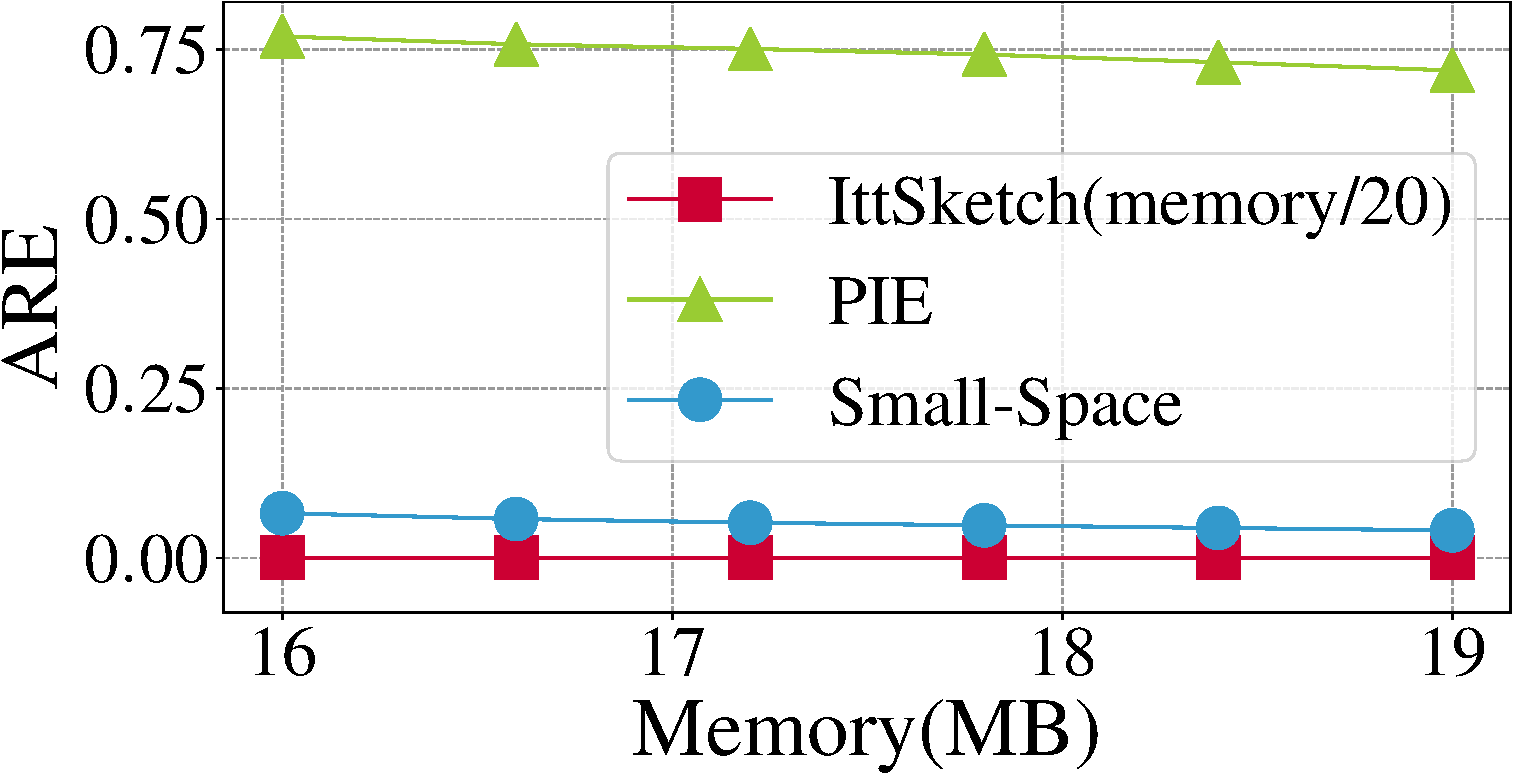
\includegraphics[width=0.95\textwidth, ]{Figures/per/per_are/per_syn_are-cropped.pdf}
		\end{center}
		}
		\postfig 
		\adjustfigs
		\prefigcaption
		\label{per_are_syn}
		\postfigcaption
		\end{minipage}
	}
	%
	\subfigure[IP trace]{
		\begin{minipage}[t]{0.225\textwidth}{
		\prefig
		\begin{center}
		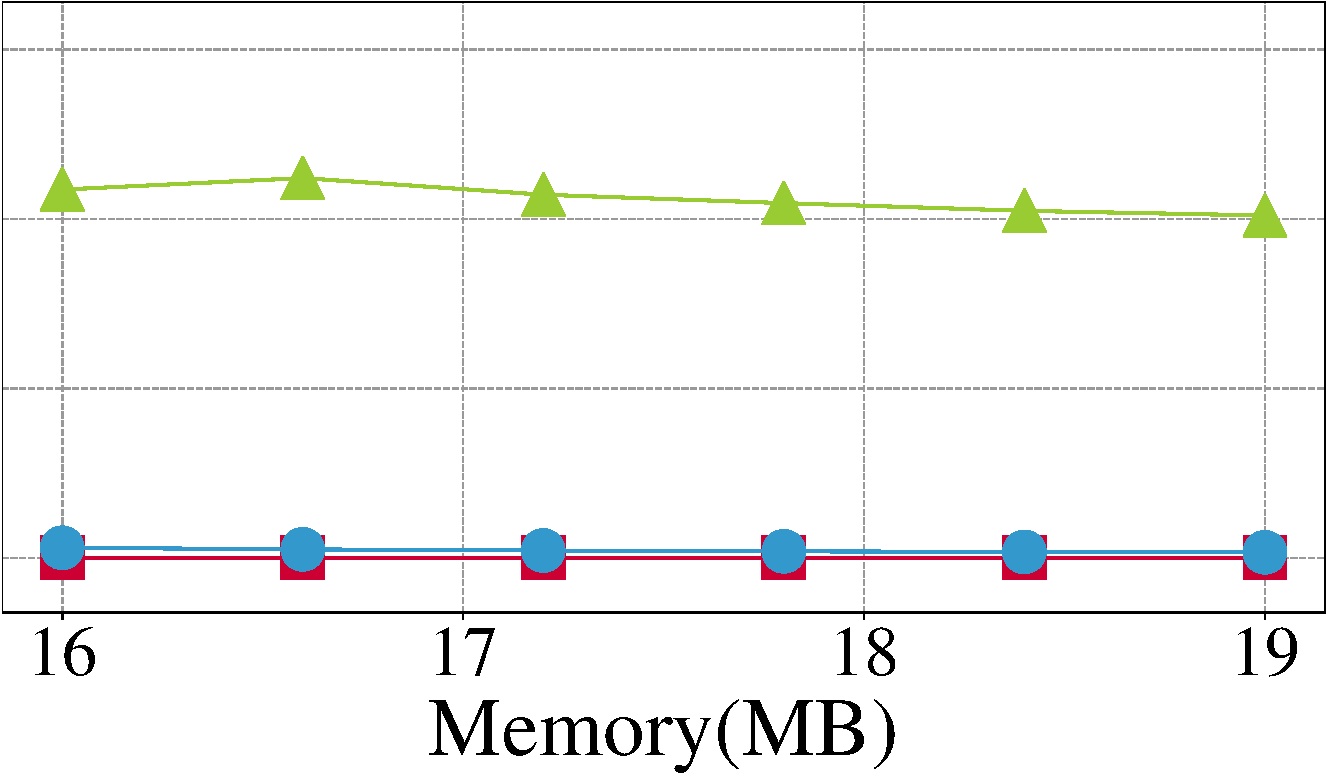
\includegraphics[width=0.95\textwidth, ]{Figures/per/per_are/per_ip_are-cropped.pdf}
		\end{center}
		}
		\postfig
		\adjustfigs
		\prefigcaption
		\label{per_are_ip}
		\postfigcaption
		\end{minipage}
	}
	%
	\subfigure[Web page]{
		\begin{minipage}[t]{0.225\textwidth}{
		\prefig
		\begin{center}		
		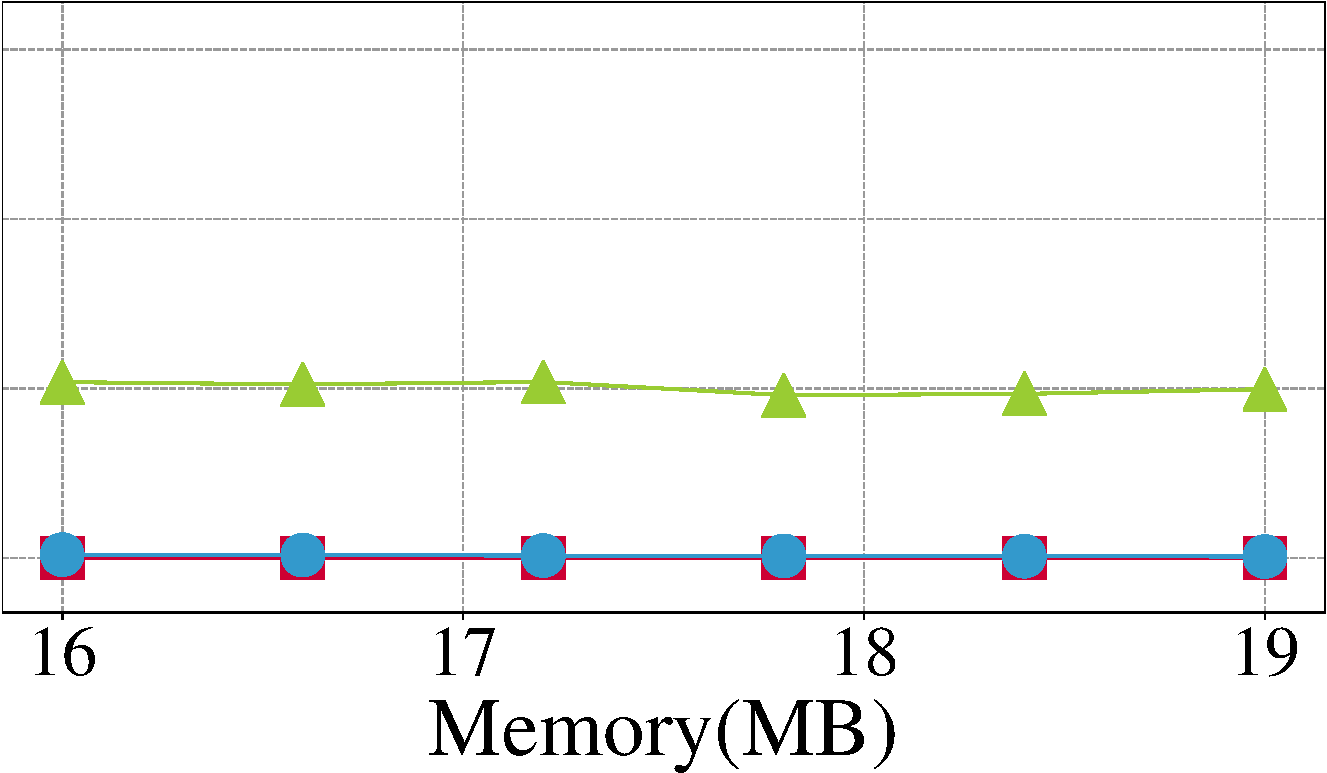
\includegraphics[width=0.95\textwidth, ]{Figures/per/per_are/per_web_are-cropped.pdf}\end{center}
		}
		\postfig 
		\adjustfigs
		\prefigcaption
		\label{per_are_web}
		\postfigcaption
		\end{minipage}
	}
	%
	\subfigure[Network dataset]{
		\begin{minipage}[t]{0.225\textwidth}{
		\prefig
		\begin{center}		
		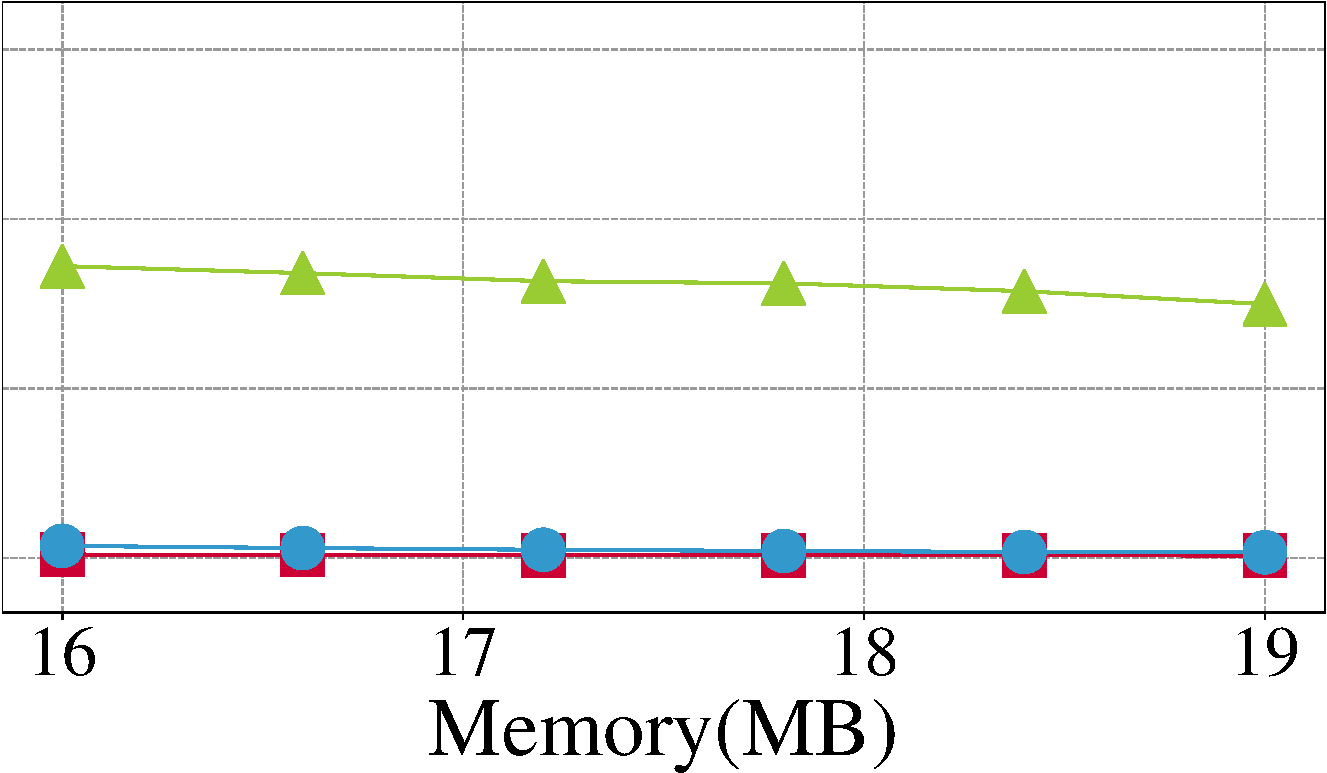
\includegraphics[width=0.95\textwidth, ]{Figures/per/per_are/per_net_are-cropped.pdf}
		\end{center}
		}
		\postfig 
		\adjustfigs
		\prefigcaption
		\label{per_are_net}
		\postfigcaption
		\end{minipage}
	}
	%
	\vvv \vvv
    \caption{ARE of finding \taskthree.}
	\label{per_are}
\end{figure*}

\begin{figure*}[!ht]
	\centering
	%
	\subfigure[Synthetic dataset]{
		\begin{minipage}[t]{0.255\textwidth}{
		\prefig
		\begin{center}
		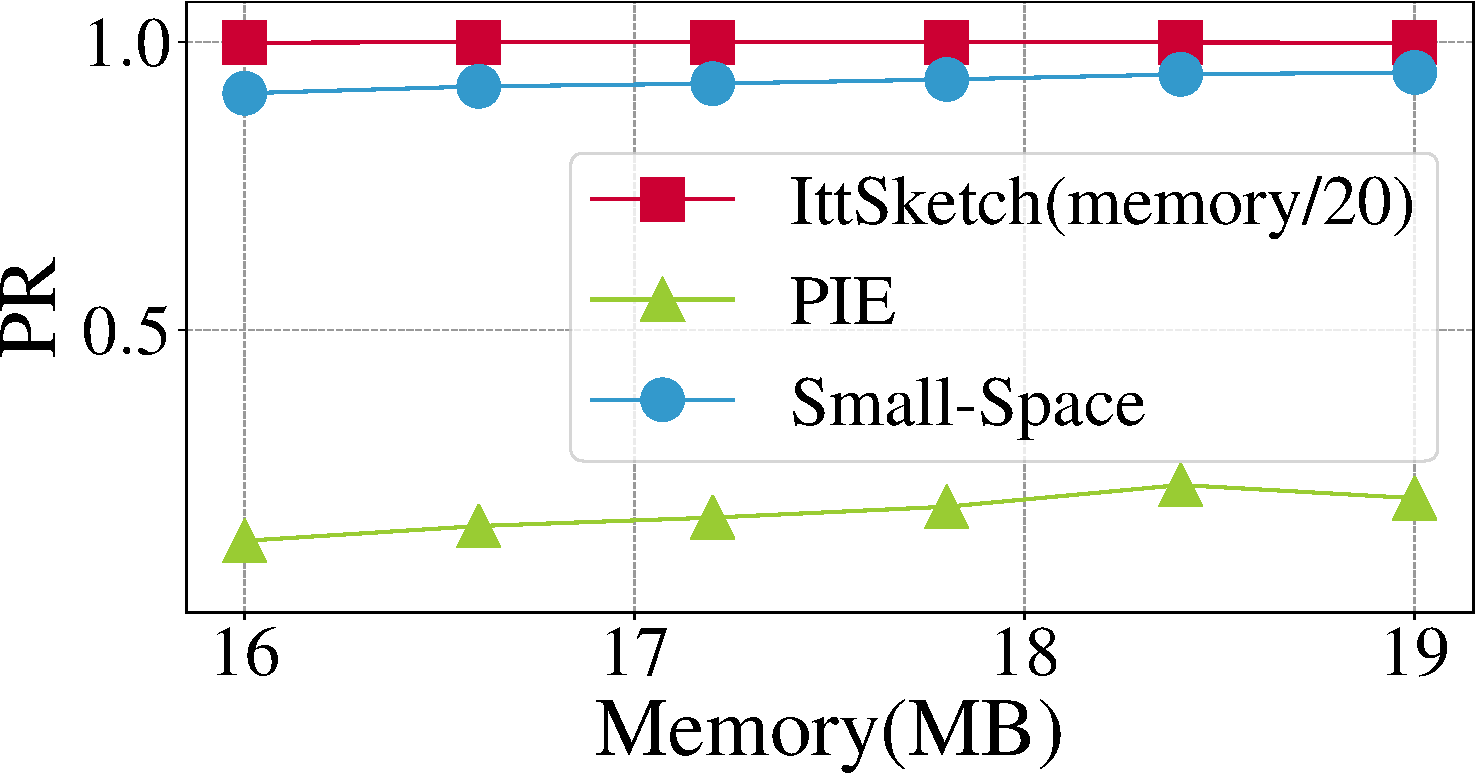
\includegraphics[width=0.95\textwidth, ]{Figures/per/per_pr/per_syn_pr-cropped.pdf}
		\end{center}
		}
		\postfig 
		\adjustfigs
		\prefigcaption
		\label{per_pr_syn}
		\postfigcaption
		\end{minipage}
	}
	%
	\subfigure[IP trace]{
		\begin{minipage}[t]{0.23\textwidth}{
		\prefig
		\begin{center}
		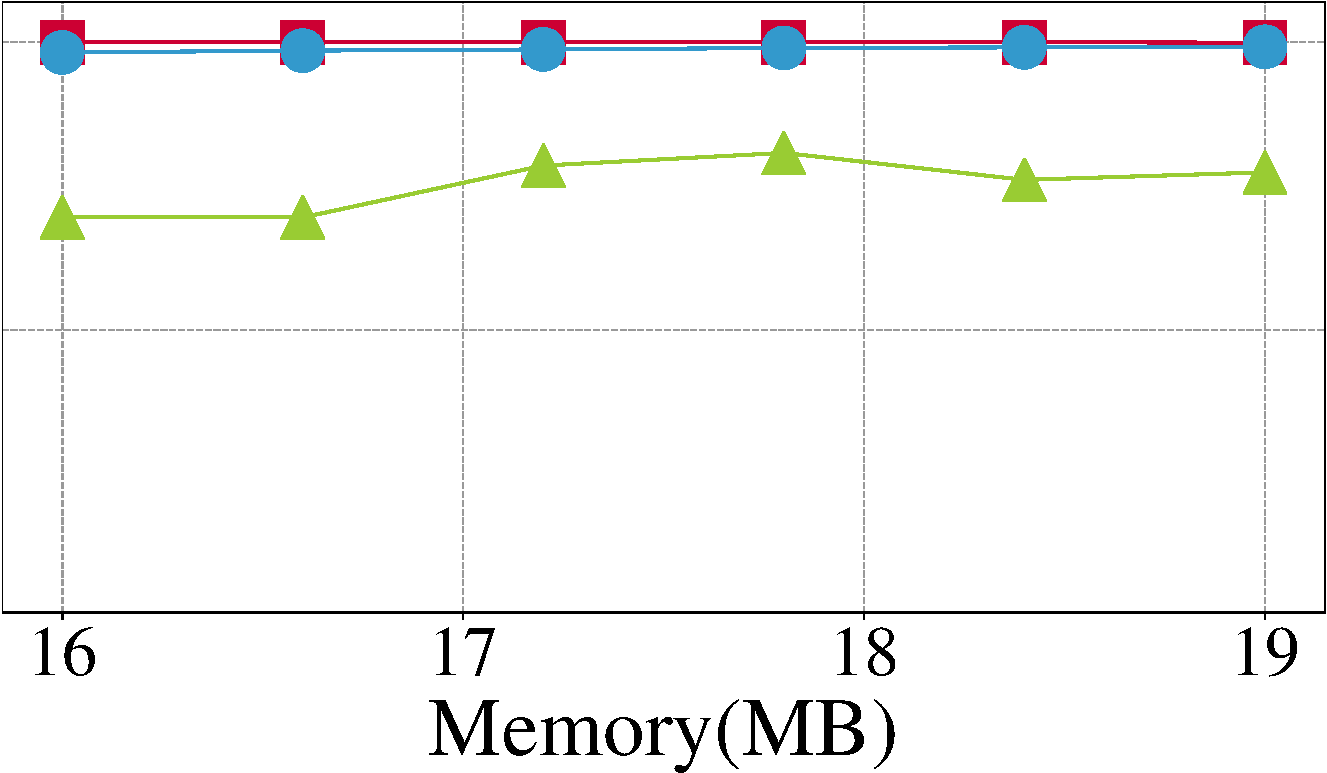
\includegraphics[width=0.95\textwidth, ]{Figures/per/per_pr/per_ip_pr-cropped.pdf}
		\end{center}
		}
		\postfig
		\adjustfigs
		\prefigcaption
		\label{per_pr_ip}
		\postfigcaption
		\end{minipage}
	}
	%
	\subfigure[Web page]{
		\begin{minipage}[t]{0.23\textwidth}{
		\prefig
		\begin{center}		
		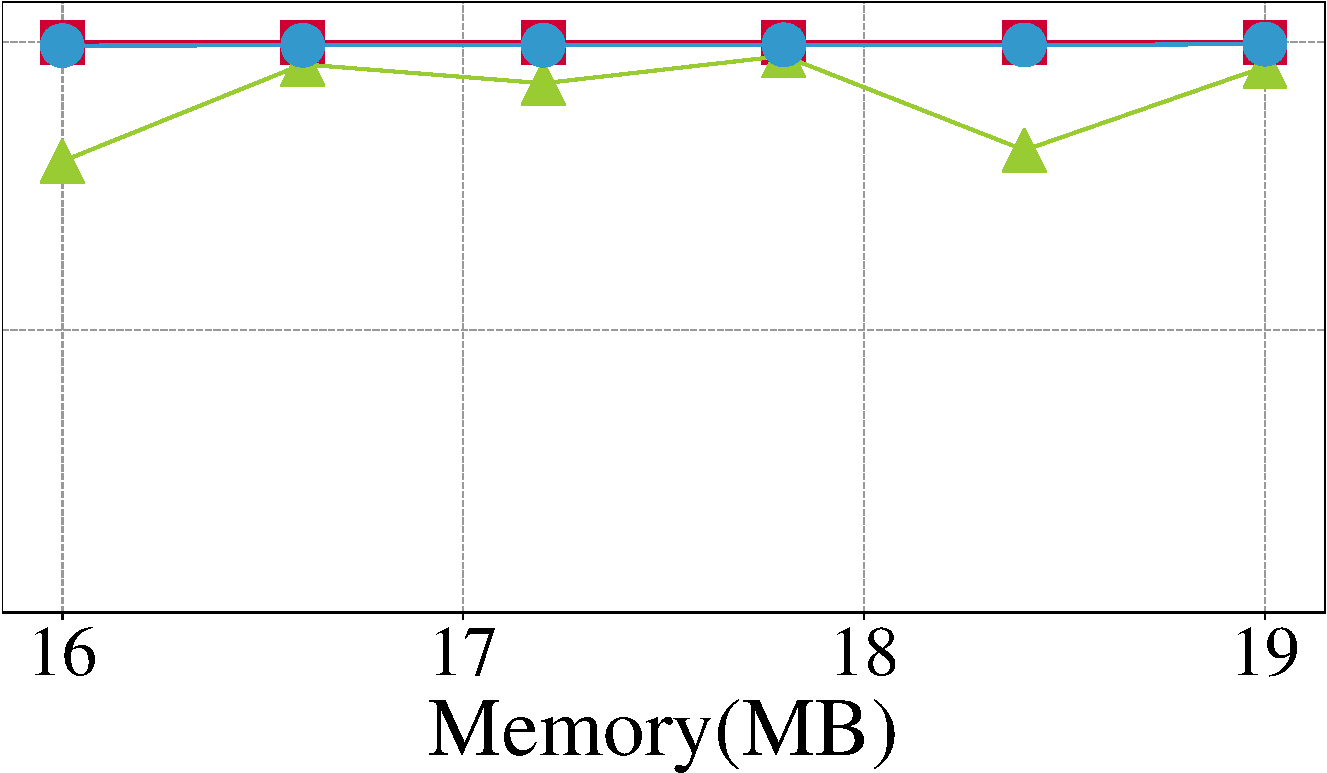
\includegraphics[width=0.95\textwidth, ]{Figures/per/per_pr/per_web_pr-cropped.pdf}
		\end{center}
		}
		\postfig 
		\adjustfigs
		\prefigcaption
		\label{per_pr_web}
		\postfigcaption
		\end{minipage}
	}
	%
	\subfigure[Network dataset]{
		\begin{minipage}[t]{0.23\textwidth}{
		\prefig
		\begin{center}		
		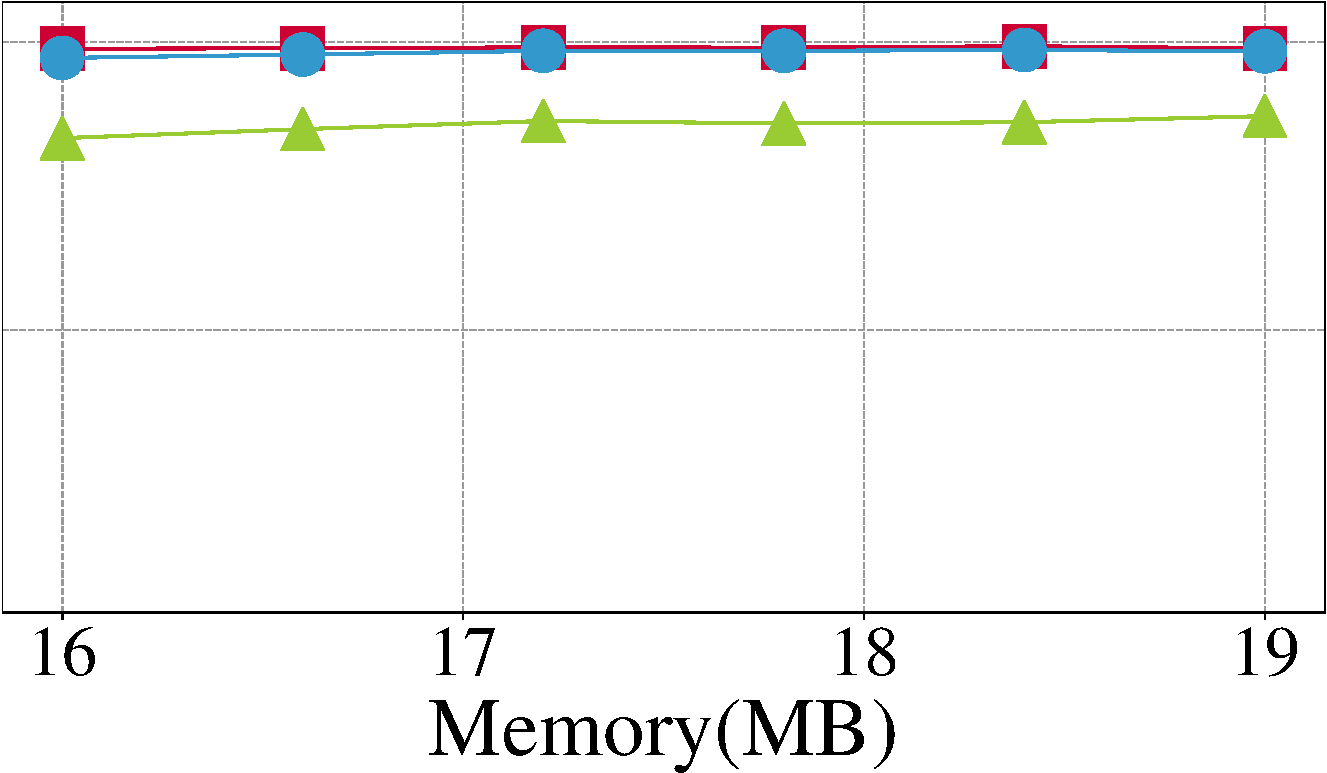
\includegraphics[width=0.95\textwidth, ]{Figures/per/per_pr/per_net_pr-cropped.pdf}
		\end{center}
		}
		\postfig 
		\adjustfigs
		\prefigcaption
		\label{per_pr_net}
		\postfigcaption
		\end{minipage}
	}
	%
	\vvv \vvv
    \caption{PR of finding \taskthree.}
	\label{per_pr}
\end{figure*}

\begin{figure*}[!ht]
	\centering
	%
	\subfigure[Synthetic dataset]{
		\begin{minipage}[t]{0.246126\textwidth}{
		\prefig
		\begin{center}
		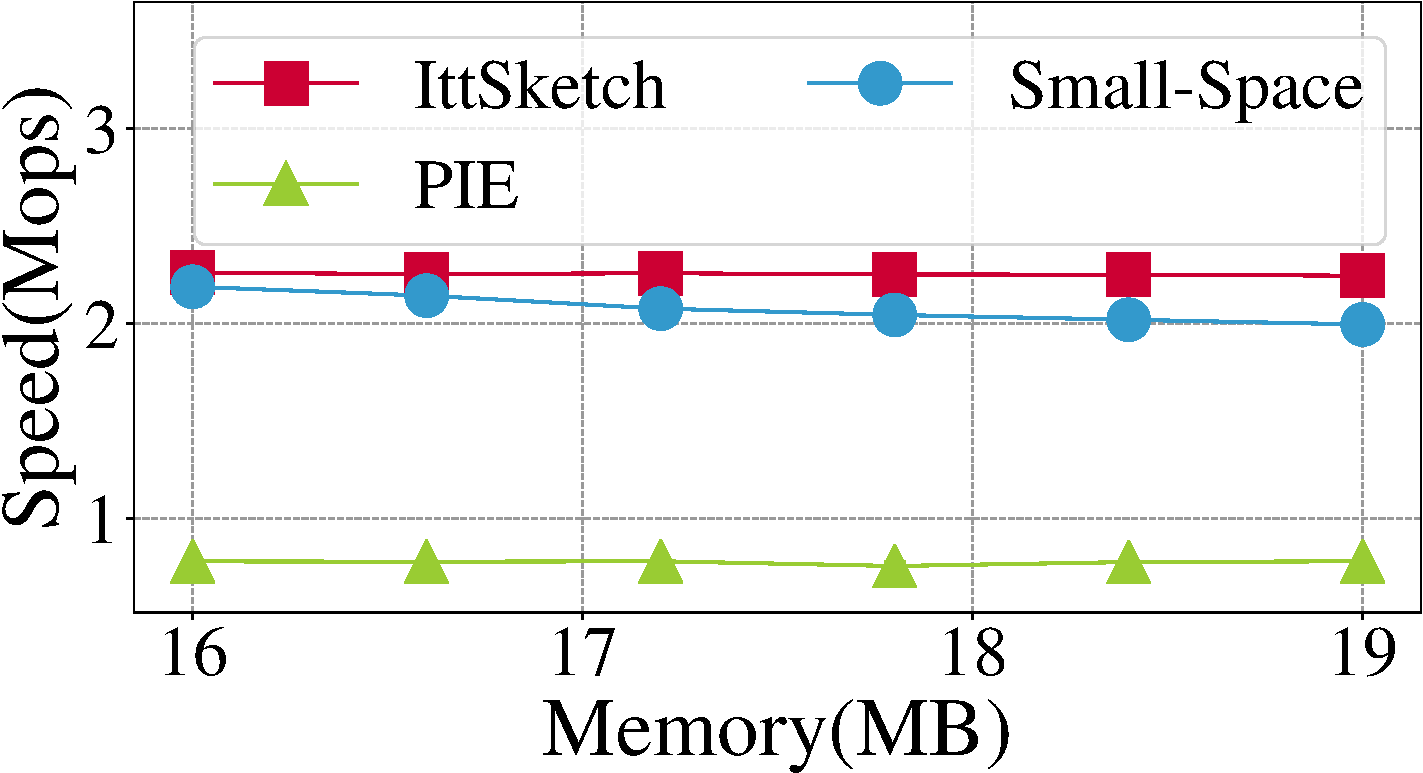
\includegraphics[width=0.95\textwidth, ]{Figures/per/per_speed/per_syn_speed-cropped.pdf}
		\end{center}
		}
		\postfig 
		\adjustfigs
		\prefigcaption
		\label{per_speed_syn}
		\postfigcaption
		\end{minipage}
	}
	%
	\subfigure[IP trace]{
		\begin{minipage}[t]{0.230622\textwidth}{
		\prefig
		\begin{center}
		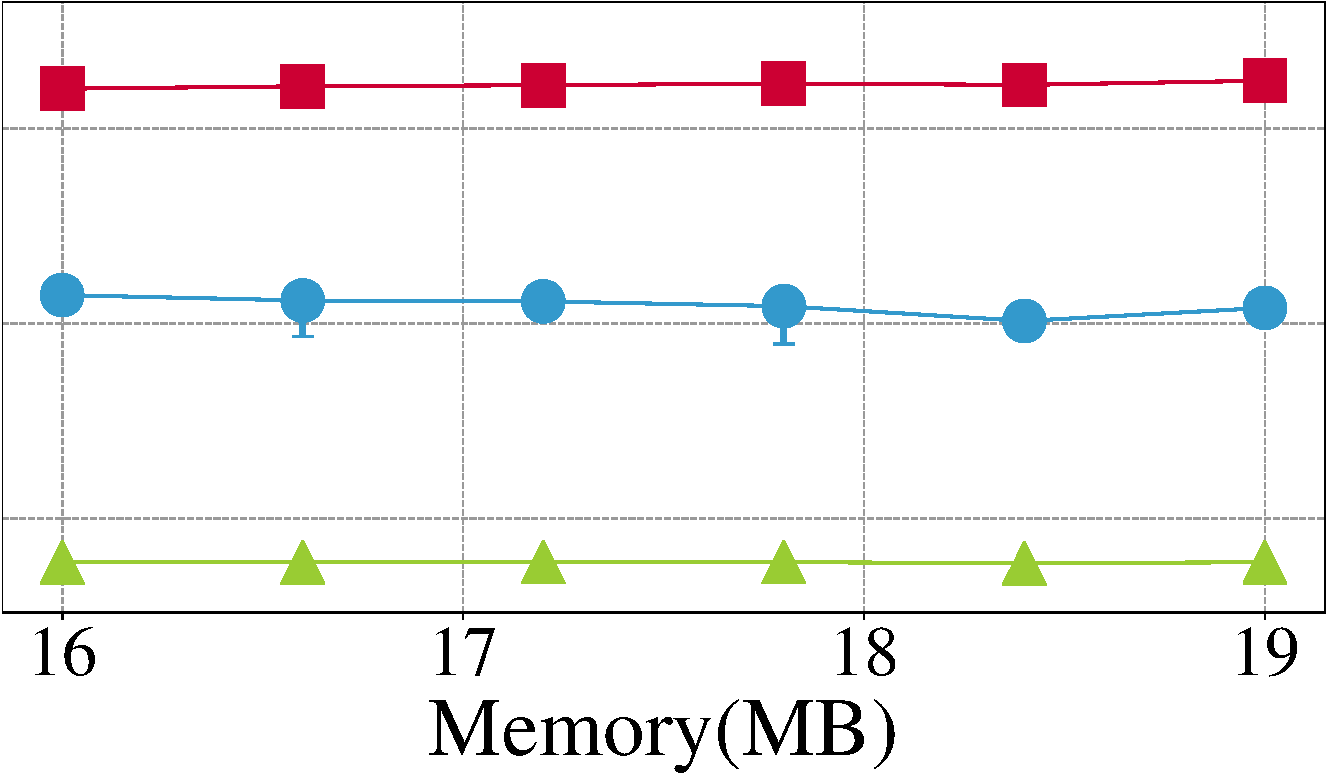
\includegraphics[width=0.95\textwidth, ]{Figures/per/per_speed/per_ip_speed-cropped.pdf}
		\end{center}
	    }
		\postfig
		\adjustfigs
		\prefigcaption
		\label{per_speed_ip}
		\postfigcaption
		\end{minipage}
	}
	%
	\subfigure[Web page]{
		\begin{minipage}[t]{0.230622\textwidth}{
		\prefig
		\begin{center}		
		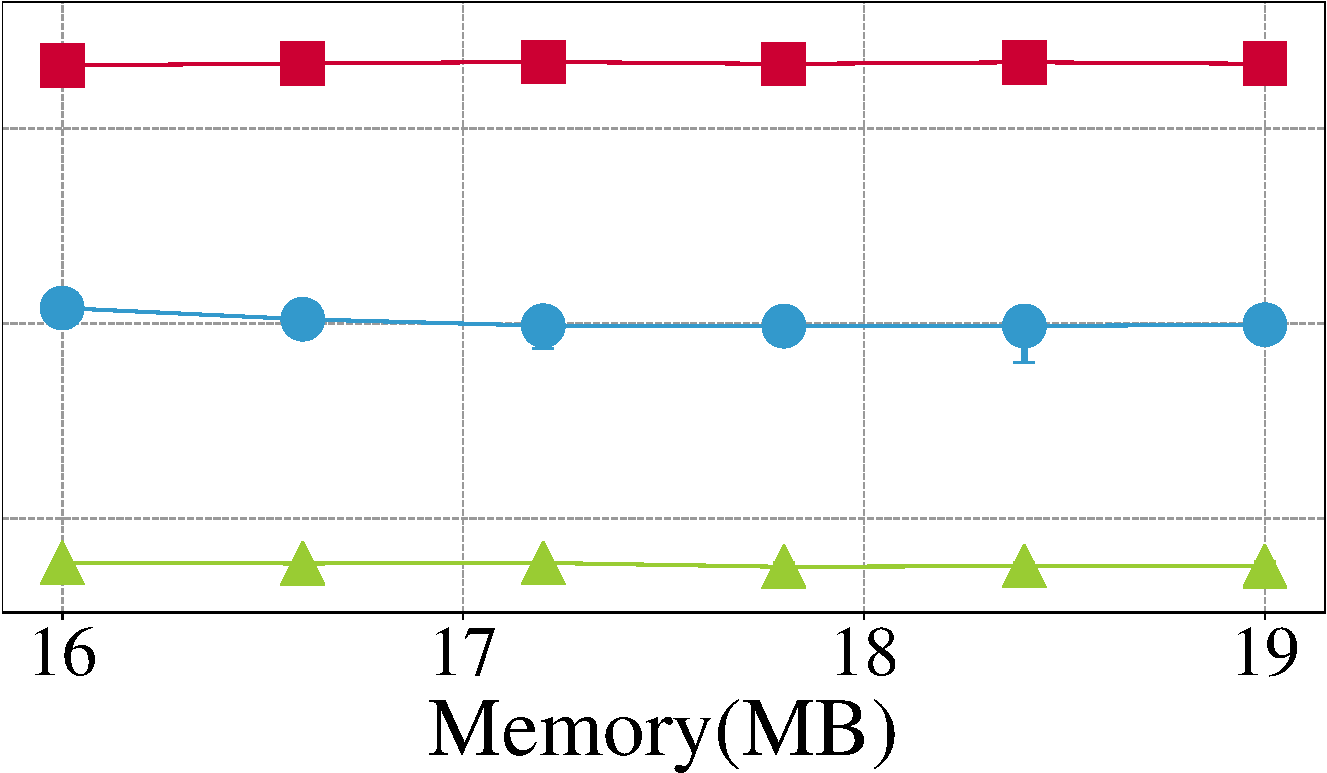
\includegraphics[width=0.95\textwidth, ]{Figures/per/per_speed/per_web_speed-cropped.pdf}
		\end{center}
		}
		\postfig 
		\adjustfigs
		\prefigcaption
		\label{per_speed_web}
		\postfigcaption
		\end{minipage}
	}
	%
	\subfigure[Network dataset]{
		\begin{minipage}[t]{0.230622\textwidth}{
		\prefig
		\begin{center}		
		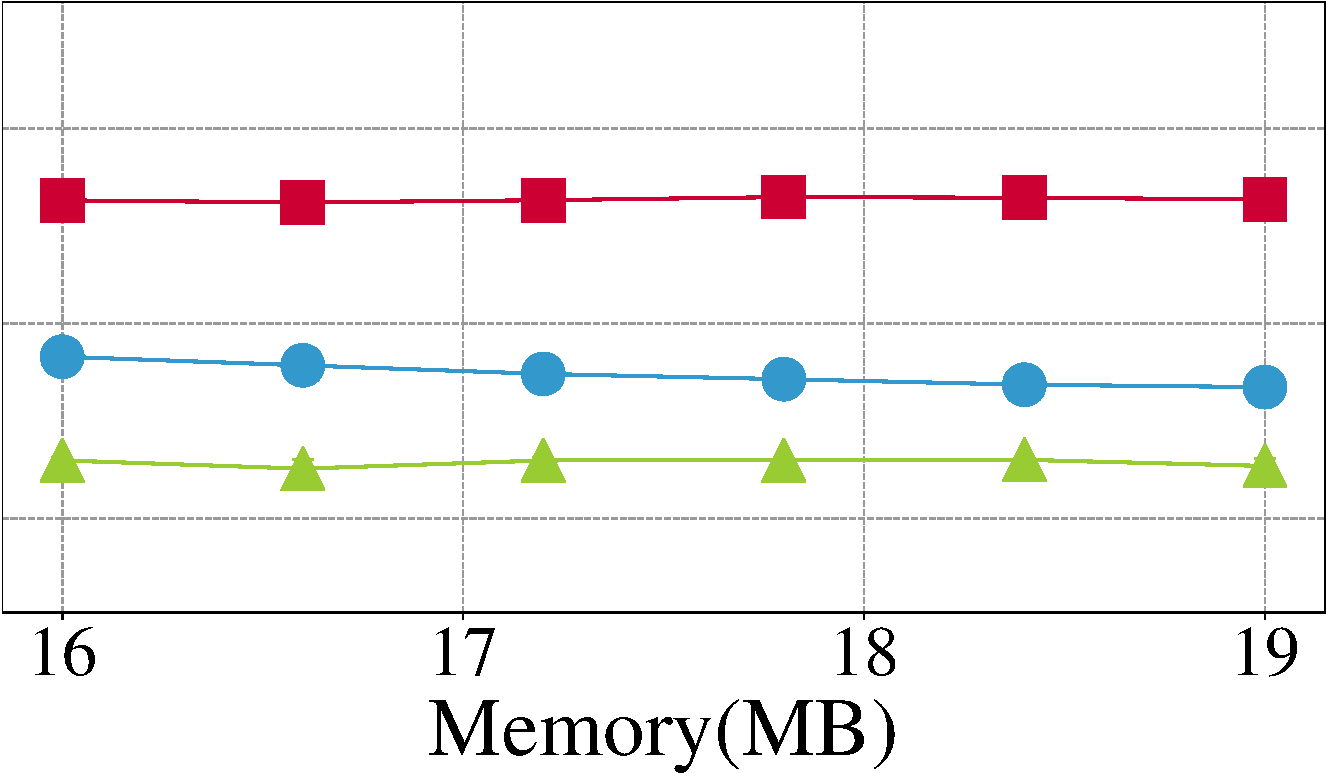
\includegraphics[width=0.95\textwidth, ]{Figures/per/per_speed/per_net_speed-cropped.pdf}
		\end{center}
		}
		\postfig 
		\adjustfigs
		\prefigcaption
		\label{per_speed_net}
		\postfigcaption
		\end{minipage}
	}
	%
	\vvv \vvv
    \caption{Speed of finding \taskthree.}
	\label{per_speed}
\end{figure*}	

%\presub
\subsection{Evaluation on Finding \tasktwo} %\postsub
\label{eva_two}

\noindent\textbf{Parameter Setting:}
%We compare three frameworks: \sketchname, \EHname and \Splittername. For each frameworks, we using CM Sketch, CM-CU Sketch and Count Sketch approaches.
%
%We compare 5 approaches: CM \sketchname, CM-CU \sketchname, Count \sketchname, \EHname {} and \Splittername.
%
%
%原则:抄袭:不能连续六个一样的单词。。。
We compare 4 algorithms: \sketchname, \supolf\cite{superspreader}, \suptlf\cite{superspreader}, and \supopen\cite{opensketch}.
Let $z$ be the number of hash functions for the Bloom filter. For \sketchname{}, we set $z=4$.
For \supolf, \suptlf{}, and \supopen, the parameters are set according to the recommendation of the authors.
In the experiment, we compare AAE, ARE, PR, CR, and insertion speed among the 4 algorithms.
The memory size ranges from 500KB to 750KB. Because other algorithms often spend much memory on the hash table or bitmap, more memory is required for the experiment. Also, we split the IP Trace Dataset into 4 sub-datasets.
			
%% why different memory size for different interest...
%% cherry picker...

\noindent\textbf{ARE (Figure~\ref{sup_are_ip}-\ref{sup_are_ip8}):}
We find that the ARE of \sketchname{} is around 31 times, 30 times, and 18 times lower than \supolf, \suptlf{}, and \supopen{}, respectively.
			
\noindent\textbf{PR (Figure~\ref{sup_pr_ip}-\ref{sup_pr_ip8}):}
We find that \sketchname{} achieves a PR above 0.99 when the memory is more than 500KB. The PR of \sketchname{} is around 4.1 times, 3.4 times, and 1.9 times higher than \supolf, \suptlf{}, and \supopen{}, respectively.
			
			
\noindent\textbf{Speed (Figure~\ref{sup_speed_ip}-\ref{sup_speed_ip8}):}
We find that, on IP Trace datasets, the insertion speed of \sketchname{} is slower than \supolf{} and \suptlf{} but is faster than \supopen{}.

\noindent\textbf{AAE (Figure~\ref{sup_aae_ip}-\ref{sup_aae_ip8}) in Appendix \ref{app:fig}:}
We find that the AAE of \sketchname{} is around 14 times, 13.3 times, and 40 times lower than \supolf, \suptlf{}, and \supopen{}, respectively.

\noindent\textbf{CR (Figure~\ref{sup_cr_ip}-\ref{sup_cr_ip8}) in Appendix \ref{app:fig}:}
We find that the CR of \sketchname{} is around 1.4 times, 1.6 times, and 1.8 times higher than \supolf, \suptlf{}, and \supopen{}, respectively.

\noindent\textbf{Summary:} 
1) \sketchname{} is more accurate than other algorithms because other algorithms often spend much memory on the hash table or bitmap, which makes them unable to count items precisely.

2) Our results show that \sketchname{} achieves both high recall rate and high precision rate. Though \supolf{} and \suptlf{} report more correct instances than \supopen{}, they also report more wrong instances due to their low sample rate, making their precision rate lower than 0.03. 